\chapter{OpenAI Codex}

\section{Engineering principles}

Codex offers interactive and noninteractive development surfaces. Use the CLI for local work, the documented SDK for programmatic workflows and app-server when an integration needs persistent interactions and event or approval handling. The current documentation is organized under ChatGPT Learn; older Codex URLs redirect there. The CLI supports workspace-scoped execution and separate approval policy settings. Skills and MCP extend available workflows; hooks are documented for supported plugin surfaces, not automatically portable to every deployment.\src{O1,O2,O3,O4,O5,O6,O8,O9}

\section{Implementation approach}

Install using the vendor distribution instructions and authenticate using an approved account or workload identity. Capture \texttt{codex -{}-version} and \texttt{codex exec -{}-help} before pinning commands. Start a disposable Git checkout, inspect instruction discovery, register only approved MCP servers, and run a read-only analysis before allowing edits. For unattended work, the example adapter uses codex exec with workspace-write and never asks for escalation; denied actions require a separate human decision. Configure the actual filesystem and network boundary outside the CLI.

\section{Verification and limitations}

Confirm the loaded policy and effective sandbox in the target OS. The examples are documentation-checked but were not live-executed. Cloud task behavior, parallel features and account entitlements must be verified separately for the intended surface.

Figure~\ref{fig:d3} illustrates the conceptual flow from Engineer / SDK to Evidence. The edges describe the proposed integration or control relationship, not undocumented internal calls.

\begin{figure}[htbp]\centering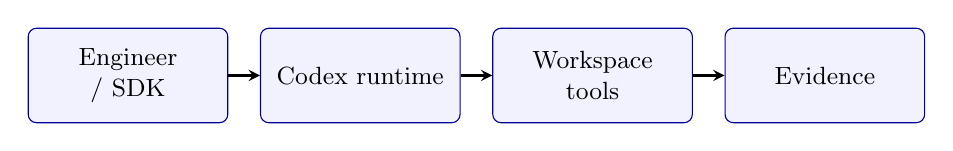
\begin{tikzpicture}[nodebox/.style={draw=blue!60!black,fill=blue!5,rounded corners=3pt,minimum height=12mm,text width=23mm,align=center,font=\small},>=stealth]
\node[nodebox] (n0) at (0.00,0.00) {Engineer / SDK};
\node[nodebox] (n1) at (2.95,0.00) {Codex runtime};
\node[nodebox] (n2) at (5.90,0.00) {Workspace tools};
\node[nodebox] (n3) at (8.85,0.00) {Evidence};
\draw[->,thick] (n0.east) -- (n1.west);
\draw[->,thick] (n1.east) -- (n2.west);
\draw[->,thick] (n2.east) -- (n3.west);
\end{tikzpicture}
\caption{Codex conceptual integration (conceptual view).}\label{fig:d3}\end{figure}

\section{Chapter conclusion}

Apply the stated verification criteria before expanding the scope of this workflow. Record deviations, evidence and unresolved risks in the task record.
